\hypertarget{bitSet_8h}{
\section{bit\-Set.h File Reference}
\label{bitSet_8h}\index{bitSet.h@{bitSet.h}}
}
{\tt \#include \char`\"{}stdio.h\char`\"{}}\par
{\tt \#include \char`\"{}stdlib.h\char`\"{}}\par
{\tt \#include \char`\"{}string.h\char`\"{}}\par


Include dependency graph for bit\-Set.h:\begin{figure}[H]
\begin{center}
\leavevmode
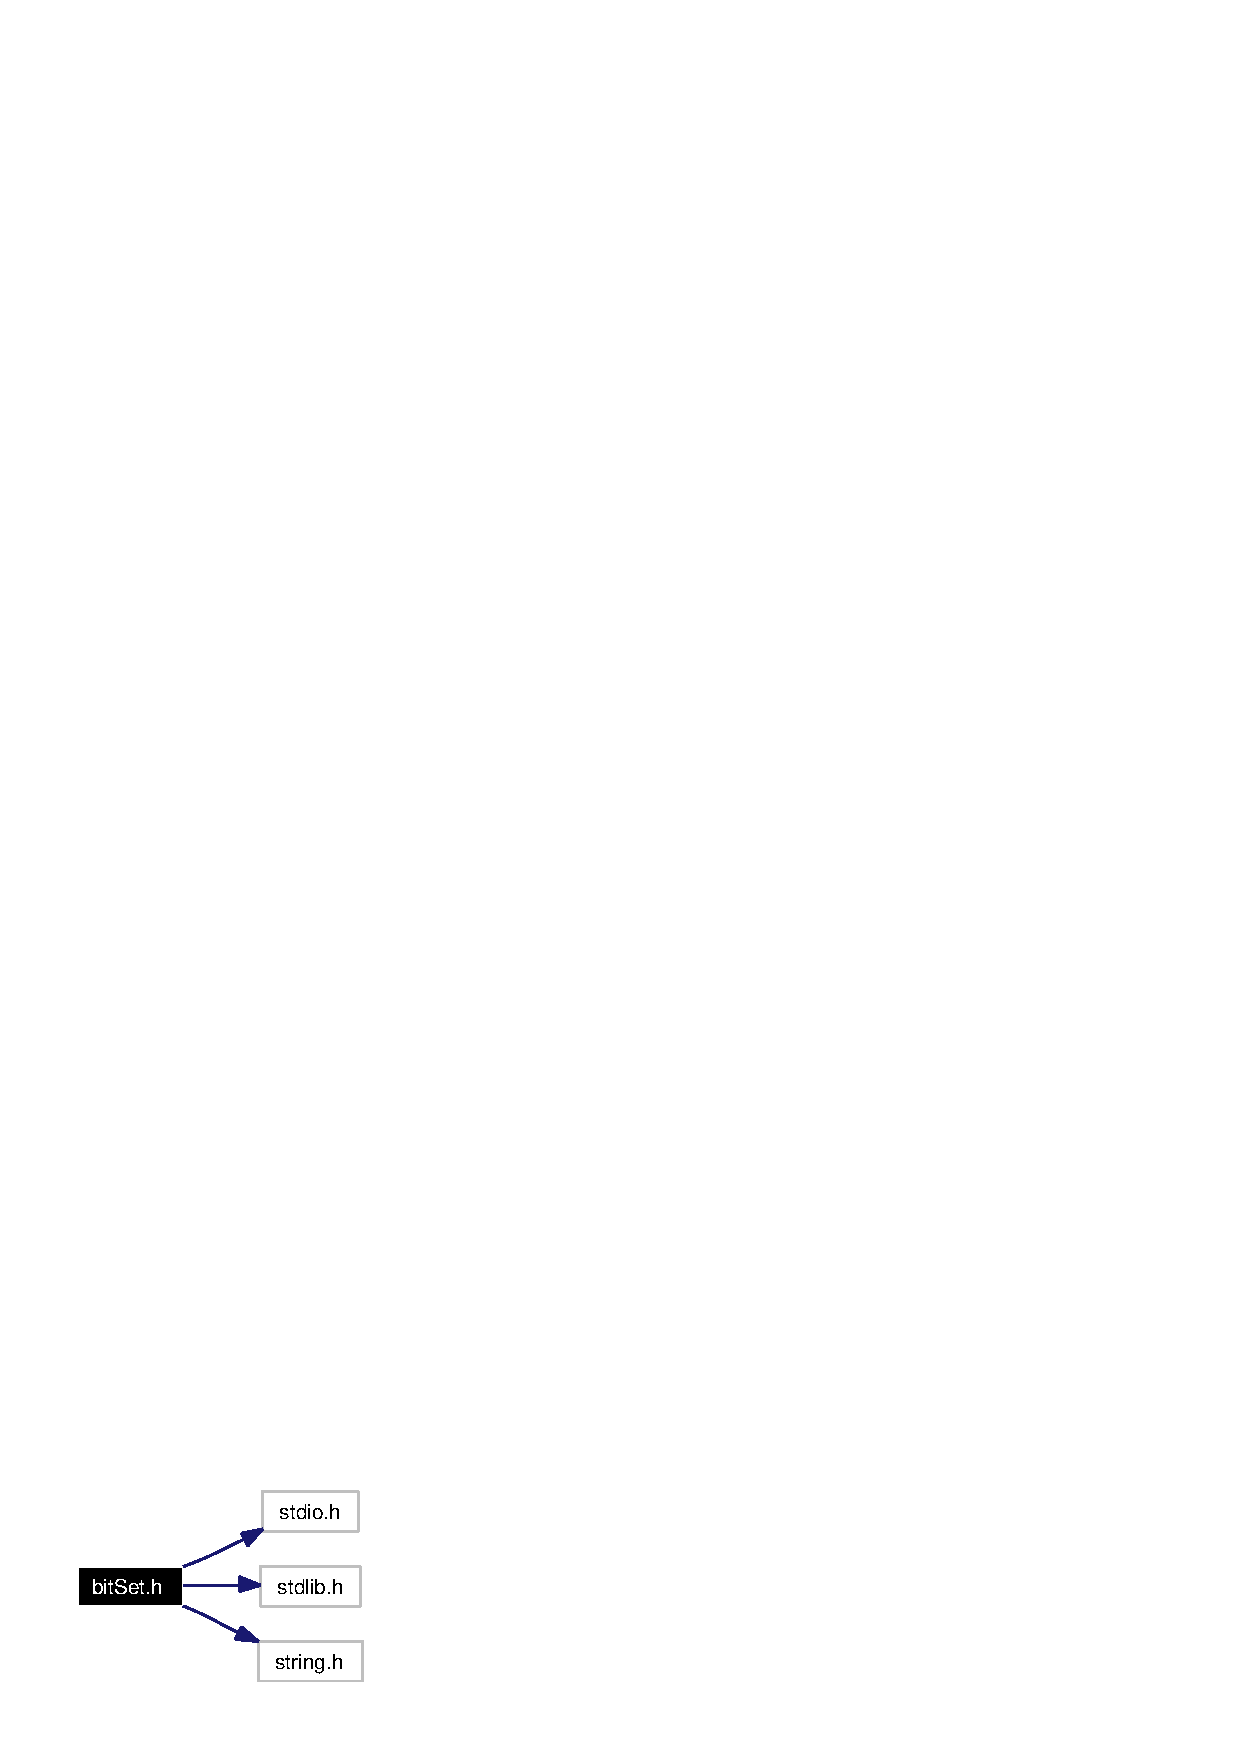
\includegraphics[width=87pt]{bitSet_8h__incl}
\end{center}
\end{figure}


This graph shows which files directly or indirectly include this file:\begin{figure}[H]
\begin{center}
\leavevmode
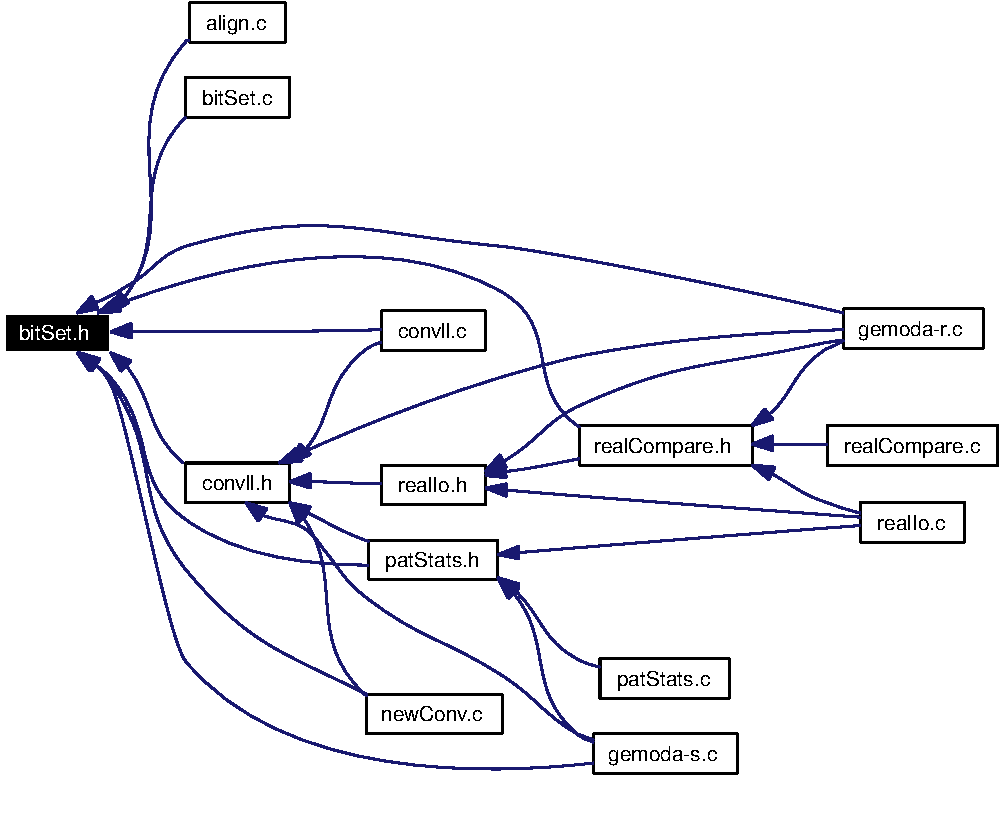
\includegraphics[width=257pt]{bitSet_8h__dep__incl}
\end{center}
\end{figure}
\subsection*{Data Structures}
\begin{CompactItemize}
\item 
struct \hyperlink{structbitSet__t}{bit\-Set\_\-t}
\item 
struct \hyperlink{structbitGraph__t}{bit\-Graph\_\-t}
\end{CompactItemize}
\subsection*{Defines}
\begin{CompactItemize}
\item 
\#define \hyperlink{bitSet_8h_a0}{BSBITSIZE}~(sizeof(\hyperlink{bitSet_8h_a9}{bit\_\-t}) $\ast$ 8)
\begin{CompactList}\small\item\em Get the size of a bit\_\-t, which is an unsigned int. \item\end{CompactList}\item 
\#define \hyperlink{bitSet_8h_a1}{BSMASK}(y)~( ((\hyperlink{bitSet_8h_a9}{bit\_\-t}) 1) $<$$<$ y \% BSBITSIZE )
\item 
\#define \hyperlink{bitSet_8h_a2}{BITSLOT}(y)~( y / BSBITSIZE )
\item 
\#define \hyperlink{bitSet_8h_a3}{BSSET}(x, y)~( x\mbox{[}BITSLOT(y)\mbox{]} $|$= BSMASK(y) )
\begin{CompactList}\small\item\em Sets the y'th bit in x (a bitset\_\-t) to be true using bitwise operators. \item\end{CompactList}\item 
\#define \hyperlink{bitSet_8h_a4}{BSCLEAR}(x, y)~( x\mbox{[}BITSLOT(y)\mbox{]} \&= $\sim$BSMASK(y) )
\begin{CompactList}\small\item\em Sets the y'th bit in x (a bitset\_\-t) to be false using bitwise operators. \item\end{CompactList}\item 
\#define \hyperlink{bitSet_8h_a5}{BSTEST}(x, y)~( x\mbox{[}BITSLOT(y)\mbox{]} \& BSMASK(y) )
\begin{CompactList}\small\item\em Tests whether the y'th bit in x (a bitset\_\-t) is true. \item\end{CompactList}\item 
\#define \hyperlink{bitSet_8h_a6}{BSNUMSLOTS}(n)~((n + BSBITSIZE - 1) / BSBITSIZE)
\item 
\#define \hyperlink{bitSet_8h_a7}{BSUNION}(x, y)~((x)$|$(y))
\begin{CompactList}\small\item\em Performs a union operation on two bit\_\-t's with bitwise operators. \item\end{CompactList}\item 
\#define \hyperlink{bitSet_8h_a8}{BSINTERSECTION}(x, y)~((x)\&(y))
\begin{CompactList}\small\item\em Performs an intersection operation on two bit\_\-t's with bitwise operators. \item\end{CompactList}\end{CompactItemize}
\subsection*{Typedefs}
\begin{CompactItemize}
\item 
typedef unsigned int \hyperlink{bitSet_8h_a9}{bit\_\-t}
\end{CompactItemize}
\subsection*{Functions}
\begin{CompactItemize}
\item 
\hyperlink{bitSet_8h_a9}{bit\_\-t} $\ast$ \hyperlink{bitSet_8h_a10}{new\-Bit\-Array} (int bytes)
\item 
\hyperlink{structbitSet__t}{bit\-Set\_\-t} $\ast$ \hyperlink{bitSet_8h_a11}{new\-Bit\-Set} (int size)
\item 
int \hyperlink{bitSet_8h_a12}{set\-True} (\hyperlink{structbitSet__t}{bit\-Set\_\-t} $\ast$s1, int x)
\item 
int \hyperlink{bitSet_8h_a13}{set\-False} (\hyperlink{structbitSet__t}{bit\-Set\_\-t} $\ast$s1, int x)
\item 
int \hyperlink{bitSet_8h_a14}{bit\-Set\-Difference} (\hyperlink{structbitSet__t}{bit\-Set\_\-t} $\ast$s1, \hyperlink{structbitSet__t}{bit\-Set\_\-t} $\ast$s2, \hyperlink{structbitSet__t}{bit\-Set\_\-t} $\ast$s3)
\item 
int \hyperlink{bitSet_8h_a15}{bit\-Set3Way\-Difference} (\hyperlink{structbitSet__t}{bit\-Set\_\-t} $\ast$s1, \hyperlink{structbitSet__t}{bit\-Set\_\-t} $\ast$s2, \hyperlink{structbitSet__t}{bit\-Set\_\-t} $\ast$s3, \hyperlink{structbitSet__t}{bit\-Set\_\-t} $\ast$s4)
\item 
int \hyperlink{bitSet_8h_a16}{bit\-Set\-Sum} (\hyperlink{structbitSet__t}{bit\-Set\_\-t} $\ast$s1, \hyperlink{structbitSet__t}{bit\-Set\_\-t} $\ast$s2, \hyperlink{structbitSet__t}{bit\-Set\_\-t} $\ast$s3)
\item 
int \hyperlink{bitSet_8h_a17}{flip\-Bits} (\hyperlink{structbitSet__t}{bit\-Set\_\-t} $\ast$s1)
\item 
int \hyperlink{bitSet_8h_a18}{fill\-Set} (\hyperlink{structbitSet__t}{bit\-Set\_\-t} $\ast$s1)
\item 
int \hyperlink{bitSet_8h_a19}{empty\-Set} (\hyperlink{structbitSet__t}{bit\-Set\_\-t} $\ast$s1)
\item 
int \hyperlink{bitSet_8h_a20}{check\-Bit} (\hyperlink{structbitSet__t}{bit\-Set\_\-t} $\ast$s1, int x)
\item 
int \hyperlink{bitSet_8h_a21}{copy\-Bit\-Graph} (\hyperlink{structbitGraph__t}{bit\-Graph\_\-t} $\ast$bg1, \hyperlink{structbitGraph__t}{bit\-Graph\_\-t} $\ast$bg2)
\item 
int \hyperlink{bitSet_8h_a22}{copy\-Set} (\hyperlink{structbitSet__t}{bit\-Set\_\-t} $\ast$s1, \hyperlink{structbitSet__t}{bit\-Set\_\-t} $\ast$s2)
\item 
int \hyperlink{bitSet_8h_a23}{delete\-Bit\-Set} (\hyperlink{structbitSet__t}{bit\-Set\_\-t} $\ast$s1)
\item 
int \hyperlink{bitSet_8h_a24}{bit\-Set\-Union} (\hyperlink{structbitSet__t}{bit\-Set\_\-t} $\ast$s1, \hyperlink{structbitSet__t}{bit\-Set\_\-t} $\ast$s2, \hyperlink{structbitSet__t}{bit\-Set\_\-t} $\ast$s3)
\item 
int \hyperlink{bitSet_8h_a25}{bit\-Set\-Intersection} (\hyperlink{structbitSet__t}{bit\-Set\_\-t} $\ast$s1, \hyperlink{structbitSet__t}{bit\-Set\_\-t} $\ast$s2, \hyperlink{structbitSet__t}{bit\-Set\_\-t} $\ast$s3)
\item 
int \hyperlink{bitSet_8h_a26}{bit\-Set3Way\-Intersection} (\hyperlink{structbitSet__t}{bit\-Set\_\-t} $\ast$s1, \hyperlink{structbitSet__t}{bit\-Set\_\-t} $\ast$s2, \hyperlink{structbitSet__t}{bit\-Set\_\-t} $\ast$s3, \hyperlink{structbitSet__t}{bit\-Set\_\-t} $\ast$s4)
\item 
int \hyperlink{bitSet_8h_a27}{count\-Set} (\hyperlink{structbitSet__t}{bit\-Set\_\-t} $\ast$s1)
\item 
int \hyperlink{bitSet_8h_a28}{fill\-Bit\-Graph} (\hyperlink{structbitGraph__t}{bit\-Graph\_\-t} $\ast$bg1)
\item 
int \hyperlink{bitSet_8h_a29}{empty\-Bit\-Graph} (\hyperlink{structbitGraph__t}{bit\-Graph\_\-t} $\ast$bg1)
\item 
int \hyperlink{bitSet_8h_a30}{print\-Bit\-Set} (\hyperlink{structbitSet__t}{bit\-Set\_\-t} $\ast$s1)
\item 
int \hyperlink{bitSet_8h_a31}{next\-Bit\-Bit\-Set} (\hyperlink{structbitSet__t}{bit\-Set\_\-t} $\ast$s1, int start)
\item 
int \hyperlink{bitSet_8h_a32}{count\-Bit\-Graph\-Non\-Zero} (\hyperlink{structbitGraph__t}{bit\-Graph\_\-t} $\ast$bg)
\item 
int \hyperlink{bitSet_8h_a33}{print\-Binary\-Bit\-Set} (\hyperlink{structbitSet__t}{bit\-Set\_\-t} $\ast$s1)
\item 
int \hyperlink{bitSet_8h_a34}{bit\-Graph\-Set\-True} (\hyperlink{structbitGraph__t}{bit\-Graph\_\-t} $\ast$bg, int x, int y)
\item 
int \hyperlink{bitSet_8h_a35}{bit\-Graph\-Set\-True\-Sym} (\hyperlink{structbitGraph__t}{bit\-Graph\_\-t} $\ast$bg, int x, int y)
\item 
int \hyperlink{bitSet_8h_a36}{bit\-Graph\-Set\-True\-Diagonal} (\hyperlink{structbitGraph__t}{bit\-Graph\_\-t} $\ast$bg)
\item 
int \hyperlink{bitSet_8h_a37}{bit\-Graph\-Set\-False\-Diagonal} (\hyperlink{structbitGraph__t}{bit\-Graph\_\-t} $\ast$bg)
\item 
int \hyperlink{bitSet_8h_a38}{print\-Bit\-Graph} (\hyperlink{structbitGraph__t}{bit\-Graph\_\-t} $\ast$bg)
\item 
\hyperlink{structbitGraph__t}{bit\-Graph\_\-t} $\ast$ \hyperlink{bitSet_8h_a39}{new\-Bit\-Graph} (int size)
\item 
int \hyperlink{bitSet_8h_a40}{delete\-Bit\-Graph} (\hyperlink{structbitGraph__t}{bit\-Graph\_\-t} $\ast$bg)
\item 
int \hyperlink{bitSet_8h_a41}{bit\-Graph\-Row\-Union} (\hyperlink{structbitGraph__t}{bit\-Graph\_\-t} $\ast$bg, int row1, int row2, \hyperlink{structbitSet__t}{bit\-Set\_\-t} $\ast$s1)
\item 
int \hyperlink{bitSet_8h_a42}{bit\-Graph\-Row\-Intersection} (\hyperlink{structbitGraph__t}{bit\-Graph\_\-t} $\ast$bg, int row1, int row2, \hyperlink{structbitSet__t}{bit\-Set\_\-t} $\ast$s1)
\item 
int \hyperlink{bitSet_8h_a43}{bit\-Graph\-Check\-Bit} (\hyperlink{structbitGraph__t}{bit\-Graph\_\-t} $\ast$bg, int x, int y)
\item 
int \hyperlink{bitSet_8h_a44}{bit\-Graph\-Set\-False\-Sym} (\hyperlink{structbitGraph__t}{bit\-Graph\_\-t} $\ast$bg, int x, int y)
\item 
int \hyperlink{bitSet_8h_a45}{bit\-Graph\-Set\-False} (\hyperlink{structbitGraph__t}{bit\-Graph\_\-t} $\ast$bg, int x, int y)
\item 
int \hyperlink{bitSet_8h_a46}{empty\-Bit\-Graph\-Row} (\hyperlink{structbitGraph__t}{bit\-Graph\_\-t} $\ast$bg, int row)
\item 
int \hyperlink{bitSet_8h_a47}{mask\-Bit\-Graph} (\hyperlink{structbitGraph__t}{bit\-Graph\_\-t} $\ast$bg1, \hyperlink{structbitSet__t}{bit\-Set\_\-t} $\ast$bs)
\end{CompactItemize}


\subsection*{Detailed Description}
This file provides declarations and definitions for a bit set object. The functions declared here are defined in \hyperlink{bitSet_8c}{bit\-Set.c}.

Definition in file \hyperlink{bitSet_8h-source}{bit\-Set.h}.

\subsection*{Define Documentation}
\hypertarget{bitSet_8h_a2}{
\index{bitSet.h@{bit\-Set.h}!BITSLOT@{BITSLOT}}
\index{BITSLOT@{BITSLOT}!bitSet.h@{bit\-Set.h}}
\subsubsection[BITSLOT]{\setlength{\rightskip}{0pt plus 5cm}\#define BITSLOT(y)~( y / BSBITSIZE )}}
\label{bitSet_8h_a2}


Finds which bit\_\-t, or \char`\"{}slot\char`\"{}, in a bitset\_\-t the y'th bit belongs to. Also used for testing single bits. 

Definition at line 71 of file bit\-Set.h.

Referenced by next\-Bit\-Bit\-Set().\hypertarget{bitSet_8h_a0}{
\index{bitSet.h@{bit\-Set.h}!BSBITSIZE@{BSBITSIZE}}
\index{BSBITSIZE@{BSBITSIZE}!bitSet.h@{bit\-Set.h}}
\subsubsection[BSBITSIZE]{\setlength{\rightskip}{0pt plus 5cm}\#define BSBITSIZE~(sizeof(\hyperlink{bitSet_8h_a9}{bit\_\-t}) $\ast$ 8)}}
\label{bitSet_8h_a0}




Definition at line 63 of file bit\-Set.h.

Referenced by next\-Bit\-Bit\-Set().\hypertarget{bitSet_8h_a4}{
\index{bitSet.h@{bit\-Set.h}!BSCLEAR@{BSCLEAR}}
\index{BSCLEAR@{BSCLEAR}!bitSet.h@{bit\-Set.h}}
\subsubsection[BSCLEAR]{\setlength{\rightskip}{0pt plus 5cm}\#define BSCLEAR(x, y)~( x\mbox{[}BITSLOT(y)\mbox{]} \&= $\sim$BSMASK(y) )}}
\label{bitSet_8h_a4}




Definition at line 77 of file bit\-Set.h.

Referenced by set\-False().\hypertarget{bitSet_8h_a8}{
\index{bitSet.h@{bit\-Set.h}!BSINTERSECTION@{BSINTERSECTION}}
\index{BSINTERSECTION@{BSINTERSECTION}!bitSet.h@{bit\-Set.h}}
\subsubsection[BSINTERSECTION]{\setlength{\rightskip}{0pt plus 5cm}\#define BSINTERSECTION(x, y)~((x)\&(y))}}
\label{bitSet_8h_a8}




Definition at line 93 of file bit\-Set.h.

Referenced by bit\-Set3Way\-Intersection(), and bit\-Set\-Intersection().\hypertarget{bitSet_8h_a1}{
\index{bitSet.h@{bit\-Set.h}!BSMASK@{BSMASK}}
\index{BSMASK@{BSMASK}!bitSet.h@{bit\-Set.h}}
\subsubsection[BSMASK]{\setlength{\rightskip}{0pt plus 5cm}\#define BSMASK(y)~( ((\hyperlink{bitSet_8h_a9}{bit\_\-t}) 1) $<$$<$ y \% BSBITSIZE )}}
\label{bitSet_8h_a1}


Uses bit operations to make a mask the size of a bit\_\-t with the y'th bit true and all other bits false. Used for testing a single bit. 

Definition at line 67 of file bit\-Set.h.\hypertarget{bitSet_8h_a6}{
\index{bitSet.h@{bit\-Set.h}!BSNUMSLOTS@{BSNUMSLOTS}}
\index{BSNUMSLOTS@{BSNUMSLOTS}!bitSet.h@{bit\-Set.h}}
\subsubsection[BSNUMSLOTS]{\setlength{\rightskip}{0pt plus 5cm}\#define BSNUMSLOTS(n)~((n + BSBITSIZE - 1) / BSBITSIZE)}}
\label{bitSet_8h_a6}


Finds the total number of bit\_\-t's (\char`\"{}slot\char`\"{}s) that are necessary for a bitset of length n. Uses integer division and supplements by BSBITSIZE - 1 to make sure that for slots that are less than full, a slot is still allocated, and for slots that are full, no extra slot is allocated. 

Definition at line 87 of file bit\-Set.h.

Referenced by new\-Bit\-Set().\hypertarget{bitSet_8h_a3}{
\index{bitSet.h@{bit\-Set.h}!BSSET@{BSSET}}
\index{BSSET@{BSSET}!bitSet.h@{bit\-Set.h}}
%\subsubsection[BSSET]{\setlength{\rightskip}{0pt plus 5cm}\#define BSSET(x, y)~( x\mbox{[}BITSLOT(y)\mbox{]} $|$= BSMASK(y) )}}
\label{bitSet_8h_a3}




Definition at line 74 of file bit\-Set.h.

Referenced by set\-True().\hypertarget{bitSet_8h_a5}{
\index{bitSet.h@{bit\-Set.h}!BSTEST@{BSTEST}}
\index{BSTEST@{BSTEST}!bitSet.h@{bit\-Set.h}}
\subsubsection[BSTEST]{\setlength{\rightskip}{0pt plus 5cm}\#define BSTEST(x, y)~( x\mbox{[}BITSLOT(y)\mbox{]} \& BSMASK(y) )}}
\label{bitSet_8h_a5}




Definition at line 80 of file bit\-Set.h.

Referenced by check\-Bit(), print\-Binary\-Bit\-Set(), and print\-Bit\-Set().\hypertarget{bitSet_8h_a7}{
\index{bitSet.h@{bit\-Set.h}!BSUNION@{BSUNION}}
\index{BSUNION@{BSUNION}!bitSet.h@{bit\-Set.h}}
\subsubsection[BSUNION]{\setlength{\rightskip}{0pt plus 5cm}\#define BSUNION(x, y)~((x)$|$(y))}}
\label{bitSet_8h_a7}




Definition at line 90 of file bit\-Set.h.

Referenced by bit\-Set\-Union().

\subsection*{Typedef Documentation}
\hypertarget{bitSet_8h_a9}{
\index{bitSet.h@{bit\-Set.h}!bit_t@{bit\_\-t}}
\index{bit_t@{bit\_\-t}!bitSet.h@{bit\-Set.h}}
\subsubsection[bit\_\-t]{\setlength{\rightskip}{0pt plus 5cm}typedef unsigned int \hyperlink{bitSet_8h_a9}{bit\_\-t}}}
\label{bitSet_8h_a9}


a bit\_\-t is the size of an unsigned integer on the current architecture.

Definition at line 15 of file bit\-Set.h.

\subsection*{Function Documentation}
\hypertarget{bitSet_8h_a43}{
\index{bitSet.h@{bit\-Set.h}!bitGraphCheckBit@{bitGraphCheckBit}}
\index{bitGraphCheckBit@{bitGraphCheckBit}!bitSet.h@{bit\-Set.h}}
\subsubsection[bitGraphCheckBit]{\setlength{\rightskip}{0pt plus 5cm}int bit\-Graph\-Check\-Bit (\hyperlink{structbitGraph__t}{bit\-Graph\_\-t} $\ast$ {\em bg}, int {\em x}, int {\em y})}}
\label{bitSet_8h_a43}


Checks the value of a bit in a \hyperlink{structbitGraph__t}{bit\-Graph\_\-t} object. Input: a \hyperlink{structbitGraph__t}{bit\-Graph\_\-t} object, the index of the row of the \hyperlink{structbitGraph__t}{bit\-Graph\_\-t} with the bit to be checked, the index of the bit in that row that is to be checked. Output: the value of the bit in the bit\-Graph being checked.

Definition at line 599 of file bit\-Set.c.

References check\-Bit(), and bit\-Graph\_\-t::graph.

Referenced by main(), and measure\-Diagonal().



\hypertarget{bitSet_8h_a42}{
\index{bitSet.h@{bit\-Set.h}!bitGraphRowIntersection@{bitGraphRowIntersection}}
\index{bitGraphRowIntersection@{bitGraphRowIntersection}!bitSet.h@{bit\-Set.h}}
\subsubsection[bitGraphRowIntersection]{\setlength{\rightskip}{0pt plus 5cm}int bit\-Graph\-Row\-Intersection (\hyperlink{structbitGraph__t}{bit\-Graph\_\-t} $\ast$ {\em bg}, int {\em row1}, int {\em row2}, \hyperlink{structbitSet__t}{bit\-Set\_\-t} $\ast$ {\em s1})}}
\label{bitSet_8h_a42}


Finds the intersection of two rows (bit\-Sets) within a \hyperlink{structbitGraph__t}{bit\-Graph\_\-t} object. Input: a \hyperlink{structbitGraph__t}{bit\-Graph\_\-t} object, first row to be compared, second row to be compared, and a \hyperlink{structbitSet__t}{bit\-Set\_\-t} to store the intersection results. Output: integer success value of 0 (and an altered destination \hyperlink{structbitSet__t}{bit\-Set\_\-t} object with a true value wherever both source bit\-Sets had a true value).

Definition at line 572 of file bit\-Set.c.

References bit\-Set\-Intersection(), and bit\-Graph\_\-t::graph.

Referenced by get\-Stat\-Mat(), and old\-Get\-Stat\-Mat().



\hypertarget{bitSet_8h_a41}{
\index{bitSet.h@{bit\-Set.h}!bitGraphRowUnion@{bitGraphRowUnion}}
\index{bitGraphRowUnion@{bitGraphRowUnion}!bitSet.h@{bit\-Set.h}}
\subsubsection[bitGraphRowUnion]{\setlength{\rightskip}{0pt plus 5cm}int bit\-Graph\-Row\-Union (\hyperlink{structbitGraph__t}{bit\-Graph\_\-t} $\ast$ {\em bg}, int {\em row1}, int {\em row2}, \hyperlink{structbitSet__t}{bit\-Set\_\-t} $\ast$ {\em s1})}}
\label{bitSet_8h_a41}


Finds the union of two rows (bit\-Sets) within a bit\-Graph Input: a \hyperlink{structbitGraph__t}{bit\-Graph\_\-t} object, first row to be compared, second row to be compared, and a \hyperlink{structbitSet__t}{bit\-Set\_\-t} to store the union results. Output: integer success value of 0 (and an altered destination \hyperlink{structbitSet__t}{bit\-Set\_\-t} object with a true value wherever one or both source bit\-Sets had a true value).

Definition at line 560 of file bit\-Set.c.

References bit\-Set\-Union(), and bit\-Graph\_\-t::graph.



\hypertarget{bitSet_8h_a45}{
\index{bitSet.h@{bit\-Set.h}!bitGraphSetFalse@{bitGraphSetFalse}}
\index{bitGraphSetFalse@{bitGraphSetFalse}!bitSet.h@{bit\-Set.h}}
\subsubsection[bitGraphSetFalse]{\setlength{\rightskip}{0pt plus 5cm}int bit\-Graph\-Set\-False (\hyperlink{structbitGraph__t}{bit\-Graph\_\-t} $\ast$ {\em bg}, int {\em x}, int {\em y})}}
\label{bitSet_8h_a45}


Sets a specific bit in a bit\-Graph false. Input: a \hyperlink{structbitGraph__t}{bit\-Graph\_\-t} object, the index of the row of the \hyperlink{structbitGraph__t}{bit\-Graph\_\-t} with the bit be set, the index of the bit in that row that is to be set. Output: integer success value of 0 (and an altered \hyperlink{structbitGraph__t}{bit\-Graph\_\-t} object).

Definition at line 623 of file bit\-Set.c.

References bit\-Graph\_\-t::graph, and set\-False().



\hypertarget{bitSet_8h_a37}{
\index{bitSet.h@{bit\-Set.h}!bitGraphSetFalseDiagonal@{bitGraphSetFalseDiagonal}}
\index{bitGraphSetFalseDiagonal@{bitGraphSetFalseDiagonal}!bitSet.h@{bit\-Set.h}}
\subsubsection[bitGraphSetFalseDiagonal]{\setlength{\rightskip}{0pt plus 5cm}int bit\-Graph\-Set\-False\-Diagonal (\hyperlink{structbitGraph__t}{bit\-Graph\_\-t} $\ast$ {\em bg})}}
\label{bitSet_8h_a37}


Sets the main diagonal of a bit\-Graph false. Input: a \hyperlink{structbitGraph__t}{bit\-Graph\_\-t} object. Output: integer success value of 0 (and an altered \hyperlink{structbitGraph__t}{bit\-Graph\_\-t} object).

Definition at line 678 of file bit\-Set.c.

References bit\-Graph\_\-t::graph, and set\-False().

Referenced by convolve().



\hypertarget{bitSet_8h_a44}{
\index{bitSet.h@{bit\-Set.h}!bitGraphSetFalseSym@{bitGraphSetFalseSym}}
\index{bitGraphSetFalseSym@{bitGraphSetFalseSym}!bitSet.h@{bit\-Set.h}}
\subsubsection[bitGraphSetFalseSym]{\setlength{\rightskip}{0pt plus 5cm}int bit\-Graph\-Set\-False\-Sym (\hyperlink{structbitGraph__t}{bit\-Graph\_\-t} $\ast$ {\em bg}, int {\em x}, int {\em y})}}
\label{bitSet_8h_a44}


Sets a specific bit and its symmetric opposite in a bit\-Graph false. For instance, given that we wanted to set the 3rd bit in the 5th row false, this would also set the 5th bit in the 3rd row. Input: a \hyperlink{structbitGraph__t}{bit\-Graph\_\-t} object, the index of the row of the bit\-Graph with the bit be set, the index of the bit in that row that is to be set. Output: integer success value of 0 (and an altered \hyperlink{structbitGraph__t}{bit\-Graph\_\-t} object).

Definition at line 637 of file bit\-Set.c.

References bit\-Graph\_\-t::graph, and set\-False().



\hypertarget{bitSet_8h_a34}{
\index{bitSet.h@{bit\-Set.h}!bitGraphSetTrue@{bitGraphSetTrue}}
\index{bitGraphSetTrue@{bitGraphSetTrue}!bitSet.h@{bit\-Set.h}}
\subsubsection[bitGraphSetTrue]{\setlength{\rightskip}{0pt plus 5cm}int bit\-Graph\-Set\-True (\hyperlink{structbitGraph__t}{bit\-Graph\_\-t} $\ast$ {\em bg}, int {\em x}, int {\em y})}}
\label{bitSet_8h_a34}


Sets a specific bit in a bit\-Graph true. Input: a \hyperlink{structbitGraph__t}{bit\-Graph\_\-t} object, the index of the row of the \hyperlink{structbitGraph__t}{bit\-Graph\_\-t} with the bit be set, the index of the bit in that row that is to be set. Output: integer success value of 0 (and an altered \hyperlink{structbitGraph__t}{bit\-Graph\_\-t} object).

Definition at line 611 of file bit\-Set.c.

References bit\-Graph\_\-t::graph, and set\-True().



\hypertarget{bitSet_8h_a36}{
\index{bitSet.h@{bit\-Set.h}!bitGraphSetTrueDiagonal@{bitGraphSetTrueDiagonal}}
\index{bitGraphSetTrueDiagonal@{bitGraphSetTrueDiagonal}!bitSet.h@{bit\-Set.h}}
\subsubsection[bitGraphSetTrueDiagonal]{\setlength{\rightskip}{0pt plus 5cm}int bit\-Graph\-Set\-True\-Diagonal (\hyperlink{structbitGraph__t}{bit\-Graph\_\-t} $\ast$ {\em bg})}}
\label{bitSet_8h_a36}


Sets the main diagonal of a bit\-Graph true. Input: a \hyperlink{structbitGraph__t}{bit\-Graph\_\-t} object. Output: integer success value of 0 (and an altered \hyperlink{structbitGraph__t}{bit\-Graph\_\-t} object).

Definition at line 664 of file bit\-Set.c.

References bit\-Graph\_\-t::graph, and set\-True().



\hypertarget{bitSet_8h_a35}{
\index{bitSet.h@{bit\-Set.h}!bitGraphSetTrueSym@{bitGraphSetTrueSym}}
\index{bitGraphSetTrueSym@{bitGraphSetTrueSym}!bitSet.h@{bit\-Set.h}}
\subsubsection[bitGraphSetTrueSym]{\setlength{\rightskip}{0pt plus 5cm}int bit\-Graph\-Set\-True\-Sym (\hyperlink{structbitGraph__t}{bit\-Graph\_\-t} $\ast$ {\em bg}, int {\em x}, int {\em y})}}
\label{bitSet_8h_a35}


Sets a specific bit and its symmetric opposite in a bit\-Graph true. For instance, given that we wanted to set the 3rd bit in the 5th row true, this would also set the 5th bit in the 3rd row. Input: a bit\-Graph, the index of the row of the bit\-Graph with the bit be set, the index of the bit in that row that is to be set. Output: integer success value of 0 (and an altered \hyperlink{structbitGraph__t}{bit\-Graph\_\-t} object).

Definition at line 652 of file bit\-Set.c.

References bit\-Graph\_\-t::graph, and set\-True().

Referenced by align\-Words\-Mat\_\-bit(), main(), and real\-Comparison().



\hypertarget{bitSet_8h_a15}{
\index{bitSet.h@{bit\-Set.h}!bitSet3WayDifference@{bitSet3WayDifference}}
\index{bitSet3WayDifference@{bitSet3WayDifference}!bitSet.h@{bit\-Set.h}}
\subsubsection[bitSet3WayDifference]{\setlength{\rightskip}{0pt plus 5cm}int bit\-Set3Way\-Difference (\hyperlink{structbitSet__t}{bit\-Set\_\-t} $\ast$ {\em s1}, \hyperlink{structbitSet__t}{bit\-Set\_\-t} $\ast$ {\em s2}, \hyperlink{structbitSet__t}{bit\-Set\_\-t} $\ast$ {\em s3}, \hyperlink{structbitSet__t}{bit\-Set\_\-t} $\ast$ {\em s4})}}
\label{bitSet_8h_a15}


\hypertarget{bitSet_8h_a26}{
\index{bitSet.h@{bit\-Set.h}!bitSet3WayIntersection@{bitSet3WayIntersection}}
\index{bitSet3WayIntersection@{bitSet3WayIntersection}!bitSet.h@{bit\-Set.h}}
\subsubsection[bitSet3WayIntersection]{\setlength{\rightskip}{0pt plus 5cm}int bit\-Set3Way\-Intersection (\hyperlink{structbitSet__t}{bit\-Set\_\-t} $\ast$ {\em s1}, \hyperlink{structbitSet__t}{bit\-Set\_\-t} $\ast$ {\em s2}, \hyperlink{structbitSet__t}{bit\-Set\_\-t} $\ast$ {\em s3}, \hyperlink{structbitSet__t}{bit\-Set\_\-t} $\ast$ {\em s4})}}
\label{bitSet_8h_a26}


Finds the intersection of 3 bit\-Sets. Input: First bit\-Set to be intersected, second bitset to be intersected. third bit\-Set to be intersected, a bit\-Set to store the result of the intersection. Output: Integer success value of 0 (and an altered destination \hyperlink{structbitSet__t}{bit\-Set\_\-t} object with a true where all three source bit\-Sets had a true.)

Definition at line 304 of file bit\-Set.c.

References BSINTERSECTION, bit\-Set\_\-t::slots, and bit\-Set\_\-t::tf.



\hypertarget{bitSet_8h_a14}{
\index{bitSet.h@{bit\-Set.h}!bitSetDifference@{bitSetDifference}}
\index{bitSetDifference@{bitSetDifference}!bitSet.h@{bit\-Set.h}}
\subsubsection[bitSetDifference]{\setlength{\rightskip}{0pt plus 5cm}int bit\-Set\-Difference (\hyperlink{structbitSet__t}{bit\-Set\_\-t} $\ast$ {\em s1}, \hyperlink{structbitSet__t}{bit\-Set\_\-t} $\ast$ {\em s2}, \hyperlink{structbitSet__t}{bit\-Set\_\-t} $\ast$ {\em s3})}}
\label{bitSet_8h_a14}


Locates all differences between two bit\-Sets. The result bit\-Set contains a true at a given bit if the two source bit\-Sets differ at that bit. Input: first bit set to be compared, second bit set to be compared. third bit set to store the results Output: integer success value of 0 (and an altered destination \hyperlink{structbitSet__t}{bit\-Set\_\-t} object with a true where the two source bit sets differed).

Definition at line 237 of file bit\-Set.c.

References bit\-Set\_\-t::slots, and bit\-Set\_\-t::tf.



\hypertarget{bitSet_8h_a25}{
\index{bitSet.h@{bit\-Set.h}!bitSetIntersection@{bitSetIntersection}}
\index{bitSetIntersection@{bitSetIntersection}!bitSet.h@{bit\-Set.h}}
\subsubsection[bitSetIntersection]{\setlength{\rightskip}{0pt plus 5cm}int bit\-Set\-Intersection (\hyperlink{structbitSet__t}{bit\-Set\_\-t} $\ast$ {\em s1}, \hyperlink{structbitSet__t}{bit\-Set\_\-t} $\ast$ {\em s2}, \hyperlink{structbitSet__t}{bit\-Set\_\-t} $\ast$ {\em s3})}}
\label{bitSet_8h_a25}


Finds the intersection of two bitsets. Input: First bit\-Set to be intersected, second bit\-Set to be intersected. a bit\-Set to store the result of the intersection. Output: Integer success value of 0 (and an altered destination \hyperlink{structbitSet__t}{bit\-Set\_\-t} object. with a true where both source bit\-Sets had a true).

Definition at line 278 of file bit\-Set.c.

References BSINTERSECTION, bit\-Set\_\-t::slots, and bit\-Set\_\-t::tf.

Referenced by bit\-Graph\-Row\-Intersection(), find\-Cliques(), and mask\-Bit\-Graph().



\hypertarget{bitSet_8h_a16}{
\index{bitSet.h@{bit\-Set.h}!bitSetSum@{bitSetSum}}
\index{bitSetSum@{bitSetSum}!bitSet.h@{bit\-Set.h}}
\subsubsection[bitSetSum]{\setlength{\rightskip}{0pt plus 5cm}int bit\-Set\-Sum (\hyperlink{structbitSet__t}{bit\-Set\_\-t} $\ast$ {\em s1}, \hyperlink{structbitSet__t}{bit\-Set\_\-t} $\ast$ {\em s2}, \hyperlink{structbitSet__t}{bit\-Set\_\-t} $\ast$ {\em s3})}}
\label{bitSet_8h_a16}


Adds two \hyperlink{structbitSet__t}{bit\-Set\_\-t} objects together. Currently unknown functionality, not used in existing code.

Definition at line 256 of file bit\-Set.c.

References bit\-Set\_\-t::slots, and bit\-Set\_\-t::tf.



\hypertarget{bitSet_8h_a24}{
\index{bitSet.h@{bit\-Set.h}!bitSetUnion@{bitSetUnion}}
\index{bitSetUnion@{bitSetUnion}!bitSet.h@{bit\-Set.h}}
\subsubsection[bitSetUnion]{\setlength{\rightskip}{0pt plus 5cm}int bit\-Set\-Union (\hyperlink{structbitSet__t}{bit\-Set\_\-t} $\ast$ {\em s1}, \hyperlink{structbitSet__t}{bit\-Set\_\-t} $\ast$ {\em s2}, \hyperlink{structbitSet__t}{bit\-Set\_\-t} $\ast$ {\em s3})}}
\label{bitSet_8h_a24}


Finds the union of two bit\-Sets Input: first bit set for the union, second bit set for the union. a bit set in which to store the results Output: an integer success value of 0 (and an altered third \hyperlink{structbitSet__t}{bit\-Set\_\-t} with the results of the union.

Definition at line 175 of file bit\-Set.c.

References BSUNION, bit\-Set\_\-t::slots, and bit\-Set\_\-t::tf.

Referenced by bit\-Graph\-Row\-Union(), and single\-Linkage().



\hypertarget{bitSet_8h_a20}{
\index{bitSet.h@{bit\-Set.h}!checkBit@{checkBit}}
\index{checkBit@{checkBit}!bitSet.h@{bit\-Set.h}}
\subsubsection[checkBit]{\setlength{\rightskip}{0pt plus 5cm}int check\-Bit (\hyperlink{structbitSet__t}{bit\-Set\_\-t} $\ast$ {\em s1}, int {\em x})}}
\label{bitSet_8h_a20}


Finds the value of a specific bit in a bit\-Set. Input: a bit\-Set, the number of the bit being queried. Output: the value of the bit being queried (1 or 0).

Definition at line 143 of file bit\-Set.c.

References BSTEST, and bit\-Set\_\-t::tf.

Referenced by bit\-Graph\-Check\-Bit(), find\-Cliques(), get\-Stat\-Mat(), mask\-Bit\-Graph(), next\-Bit\-Bit\-Set(), single\-Linkage(), and whole\-Round\-Conv().



\hypertarget{bitSet_8h_a21}{
\index{bitSet.h@{bit\-Set.h}!copyBitGraph@{copyBitGraph}}
\index{copyBitGraph@{copyBitGraph}!bitSet.h@{bit\-Set.h}}
\subsubsection[copyBitGraph]{\setlength{\rightskip}{0pt plus 5cm}int copy\-Bit\-Graph (\hyperlink{structbitGraph__t}{bit\-Graph\_\-t} $\ast$ {\em bg1}, \hyperlink{structbitGraph__t}{bit\-Graph\_\-t} $\ast$ {\em bg2})}}
\label{bitSet_8h_a21}


Copies the true/false contents of one bit graph into an existing bit graph. Both bit graphs must be the same size, and each corresponding bit set between the two bit graphs must be the same size. Input: source bit graph, destination \hyperlink{structbitGraph__t}{bit\-Graph\_\-t} object. Output: integer success value of 0 (and an altered destination bit graph).

Definition at line 215 of file bit\-Set.c.

References copy\-Set(), bit\-Graph\_\-t::graph, and bit\-Graph\_\-t::size.



\hypertarget{bitSet_8h_a22}{
\index{bitSet.h@{bit\-Set.h}!copySet@{copySet}}
\index{copySet@{copySet}!bitSet.h@{bit\-Set.h}}
\subsubsection[copySet]{\setlength{\rightskip}{0pt plus 5cm}int copy\-Set (\hyperlink{structbitSet__t}{bit\-Set\_\-t} $\ast$ {\em s1}, \hyperlink{structbitSet__t}{bit\-Set\_\-t} $\ast$ {\em s2})}}
\label{bitSet_8h_a22}


Copies the true/false contents of one bit set into an existing bit set. Both bit sets must be the same size. Input: source bit set, destination \hyperlink{structbitSet__t}{bit\-Set\_\-t} object. Output: integer success value of 0 (and an altered destination bitset.

Definition at line 195 of file bit\-Set.c.

References bit\-Set\_\-t::slots, and bit\-Set\_\-t::tf.

Referenced by copy\-Bit\-Graph(), filter\-Graph(), and single\-Linkage().



\hypertarget{bitSet_8h_a32}{
\index{bitSet.h@{bit\-Set.h}!countBitGraphNonZero@{countBitGraphNonZero}}
\index{countBitGraphNonZero@{countBitGraphNonZero}!bitSet.h@{bit\-Set.h}}
\subsubsection[countBitGraphNonZero]{\setlength{\rightskip}{0pt plus 5cm}int count\-Bit\-Graph\-Non\-Zero (\hyperlink{structbitGraph__t}{bit\-Graph\_\-t} $\ast$ {\em bg})}}
\label{bitSet_8h_a32}


Counts the number of true (non-zero) values in a \hyperlink{structbitGraph__t}{bit\-Graph\_\-t} object. Input: a \hyperlink{structbitGraph__t}{bit\-Graph\_\-t} object. Output: the integer number of true (non-zero) values in the \hyperlink{structbitGraph__t}{bit\-Graph\_\-t} object.

Definition at line 511 of file bit\-Set.c.

References count\-Set(), and bit\-Graph\_\-t::graph.



\hypertarget{bitSet_8h_a27}{
\index{bitSet.h@{bit\-Set.h}!countSet@{countSet}}
\index{countSet@{countSet}!bitSet.h@{bit\-Set.h}}
\subsubsection[countSet]{\setlength{\rightskip}{0pt plus 5cm}int count\-Set (\hyperlink{structbitSet__t}{bit\-Set\_\-t} $\ast$ {\em s1})}}
\label{bitSet_8h_a27}


Counts the number of true values in a bit\-Set. Input: a \hyperlink{structbitSet__t}{bit\-Set\_\-t} object. Output: number of true values in that \hyperlink{structbitSet__t}{bit\-Set\_\-t} object.

Definition at line 413 of file bit\-Set.c.

References bitcount32\_\-precomp(), and bit\-Set\_\-t::tf.

Referenced by bit\-Set\-To\-CSet(), count\-Bit\-Graph\-Non\-Zero(), filter\-Graph(), filter\-Iter(), find\-Cliques(), get\-Stat\-Mat(), old\-Get\-Stat\-Mat(), print\-Bit\-Set(), single\-Linkage(), and whole\-Clique\-Conv().



\hypertarget{bitSet_8h_a40}{
\index{bitSet.h@{bit\-Set.h}!deleteBitGraph@{deleteBitGraph}}
\index{deleteBitGraph@{deleteBitGraph}!bitSet.h@{bit\-Set.h}}
\subsubsection[deleteBitGraph]{\setlength{\rightskip}{0pt plus 5cm}int delete\-Bit\-Graph (\hyperlink{structbitGraph__t}{bit\-Graph\_\-t} $\ast$ {\em bg})}}
\label{bitSet_8h_a40}


Deletes a \hyperlink{structbitGraph__t}{bit\-Graph\_\-t} object from memory. Input: a \hyperlink{structbitGraph__t}{bit\-Graph\_\-t} object to be deleted. Output: integer success value from 0 (and deletion of a \hyperlink{structbitGraph__t}{bit\-Graph\_\-t} object).

Definition at line 799 of file bit\-Set.c.

References delete\-Bit\-Set(), and bit\-Graph\_\-t::graph.

Referenced by main().



\hypertarget{bitSet_8h_a23}{
\index{bitSet.h@{bit\-Set.h}!deleteBitSet@{deleteBitSet}}
\index{deleteBitSet@{deleteBitSet}!bitSet.h@{bit\-Set.h}}
\subsubsection[deleteBitSet]{\setlength{\rightskip}{0pt plus 5cm}int delete\-Bit\-Set (\hyperlink{structbitSet__t}{bit\-Set\_\-t} $\ast$ {\em s1})}}
\label{bitSet_8h_a23}


Performs memory management for the deletion of a \hyperlink{structbitSet__t}{bit\-Set\_\-t} structure. Input: a \hyperlink{structbitSet__t}{bit\-Set\_\-t} object. Output: integer success value of 1.

Definition at line 154 of file bit\-Set.c.

References bit\-Set\_\-t::tf.

Referenced by convolve(), delete\-Bit\-Graph(), filter\-Graph(), find\-Cliques(), get\-Stat\-Mat(), old\-Get\-Stat\-Mat(), whole\-Clique\-Conv(), and whole\-Round\-Conv().



\hypertarget{bitSet_8h_a29}{
\index{bitSet.h@{bit\-Set.h}!emptyBitGraph@{emptyBitGraph}}
\index{emptyBitGraph@{emptyBitGraph}!bitSet.h@{bit\-Set.h}}
\subsubsection[emptyBitGraph]{\setlength{\rightskip}{0pt plus 5cm}int empty\-Bit\-Graph (\hyperlink{structbitGraph__t}{bit\-Graph\_\-t} $\ast$ {\em bg1})}}
\label{bitSet_8h_a29}


Sets all bits in the \hyperlink{structbitGraph__t}{bit\-Graph\_\-t} object to false. Input: a \hyperlink{structbitGraph__t}{bit\-Graph\_\-t} object. Output: integer success value of 0 (and a \hyperlink{structbitGraph__t}{bit\-Graph\_\-t} with all false bits).

Definition at line 744 of file bit\-Set.c.

References empty\-Set(), and bit\-Graph\_\-t::graph.



\hypertarget{bitSet_8h_a46}{
\index{bitSet.h@{bit\-Set.h}!emptyBitGraphRow@{emptyBitGraphRow}}
\index{emptyBitGraphRow@{emptyBitGraphRow}!bitSet.h@{bit\-Set.h}}
\subsubsection[emptyBitGraphRow]{\setlength{\rightskip}{0pt plus 5cm}int empty\-Bit\-Graph\-Row (\hyperlink{structbitGraph__t}{bit\-Graph\_\-t} $\ast$ {\em bg}, int {\em row})}}
\label{bitSet_8h_a46}


Sets all bits in a \hyperlink{structbitGraph__t}{bit\-Graph\_\-t} row (a \hyperlink{structbitSet__t}{bit\-Set\_\-t} object) false. Input: a bit\-Graph, a row in the \hyperlink{structbitGraph__t}{bit\-Graph\_\-t} object to be emptied. Output: integer success value of 0 (and an altered \hyperlink{structbitGraph__t}{bit\-Graph\_\-t} object).

Definition at line 788 of file bit\-Set.c.

References empty\-Set(), and bit\-Graph\_\-t::graph.



\hypertarget{bitSet_8h_a19}{
\index{bitSet.h@{bit\-Set.h}!emptySet@{emptySet}}
\index{emptySet@{emptySet}!bitSet.h@{bit\-Set.h}}
\subsubsection[emptySet]{\setlength{\rightskip}{0pt plus 5cm}int empty\-Set (\hyperlink{structbitSet__t}{bit\-Set\_\-t} $\ast$ {\em s1})}}
\label{bitSet_8h_a19}


Sets all values in a bit\-Set to false. Input: a \hyperlink{structbitSet__t}{bit\-Set\_\-t} object. Output: integer success value of 1.

Definition at line 131 of file bit\-Set.c.

References bit\-Set\_\-t::bytes, and bit\-Set\_\-t::tf.

Referenced by empty\-Bit\-Graph(), empty\-Bit\-Graph\-Row(), filter\-Graph(), filter\-Iter(), mask\-Bit\-Graph(), prune\-Bit\-Graph(), and search\-Mems\-With\-List().



\hypertarget{bitSet_8h_a28}{
\index{bitSet.h@{bit\-Set.h}!fillBitGraph@{fillBitGraph}}
\index{fillBitGraph@{fillBitGraph}!bitSet.h@{bit\-Set.h}}
\subsubsection[fillBitGraph]{\setlength{\rightskip}{0pt plus 5cm}int fill\-Bit\-Graph (\hyperlink{structbitGraph__t}{bit\-Graph\_\-t} $\ast$ {\em bg1})}}
\label{bitSet_8h_a28}


Sets all bits in the \hyperlink{structbitGraph__t}{bit\-Graph\_\-t} object to true. Input: a \hyperlink{structbitGraph__t}{bit\-Graph\_\-t} object. Output: integer success value of 0 (and a \hyperlink{structbitGraph__t}{bit\-Graph\_\-t} object with all true bits).

Definition at line 730 of file bit\-Set.c.

References fill\-Set(), and bit\-Graph\_\-t::graph.



\hypertarget{bitSet_8h_a18}{
\index{bitSet.h@{bit\-Set.h}!fillSet@{fillSet}}
\index{fillSet@{fillSet}!bitSet.h@{bit\-Set.h}}
\subsubsection[fillSet]{\setlength{\rightskip}{0pt plus 5cm}int fill\-Set (\hyperlink{structbitSet__t}{bit\-Set\_\-t} $\ast$ {\em s1})}}
\label{bitSet_8h_a18}


Sets all values in a bit\-Set to true. Input: a bit\-Set. Output: integer success value of 1.

Definition at line 119 of file bit\-Set.c.

References bit\-Set\_\-t::bytes, and bit\-Set\_\-t::tf.

Referenced by convolve(), fill\-Bit\-Graph(), and whole\-Round\-Conv().



\hypertarget{bitSet_8h_a17}{
\index{bitSet.h@{bit\-Set.h}!flipBits@{flipBits}}
\index{flipBits@{flipBits}!bitSet.h@{bit\-Set.h}}
\subsubsection[flipBits]{\setlength{\rightskip}{0pt plus 5cm}int flip\-Bits (\hyperlink{structbitSet__t}{bit\-Set\_\-t} $\ast$ {\em s1})}}
\label{bitSet_8h_a17}


Inverts all values in a bit\-Set, making all trues false and all falses true. Input: a bit\-Set. Output: integer success value of 1.

Definition at line 105 of file bit\-Set.c.

References bit\-Set\_\-t::tf.



\hypertarget{bitSet_8h_a47}{
\index{bitSet.h@{bit\-Set.h}!maskBitGraph@{maskBitGraph}}
\index{maskBitGraph@{maskBitGraph}!bitSet.h@{bit\-Set.h}}
\subsubsection[maskBitGraph]{\setlength{\rightskip}{0pt plus 5cm}int mask\-Bit\-Graph (\hyperlink{structbitGraph__t}{bit\-Graph\_\-t} $\ast$ {\em bg1}, \hyperlink{structbitSet__t}{bit\-Set\_\-t} $\ast$ {\em bs})}}
\label{bitSet_8h_a47}


Makes a bit\-Graph contain only true bits according to the bitmask given. Only locations with the row and column both true in the bitmask can be true if they were initially true. If they were false, they remain false. If the location does not have both the row and the column in the bitmask, it is made false. Note, this is not currently used in Gemoda. Input: a bit\-Graph, a mask in the form of a \hyperlink{structbitSet__t}{bit\-Set\_\-t} object. Output: integer success value of 0 (and an altered \hyperlink{structbitGraph__t}{bit\-Graph\_\-t} object).

Definition at line 712 of file bit\-Set.c.

References bit\-Set\-Intersection(), check\-Bit(), empty\-Set(), and bit\-Graph\_\-t::graph.



\hypertarget{bitSet_8h_a10}{
\index{bitSet.h@{bit\-Set.h}!newBitArray@{newBitArray}}
\index{newBitArray@{newBitArray}!bitSet.h@{bit\-Set.h}}
\subsubsection[newBitArray]{\setlength{\rightskip}{0pt plus 5cm}\hyperlink{bitSet_8h_a9}{bit\_\-t}$\ast$ new\-Bit\-Array (int {\em bytes})}}
\label{bitSet_8h_a10}


Creates a bit array for use in high-throughput intersections/unions. Input: desired size of bit array in byte. Output: a new bit array in bit\_\-t forma. Note: this should not be called directly; see new\-Bit\-Set.

Definition at line 18 of file bit\-Set.c.

Referenced by new\-Bit\-Set().



\hypertarget{bitSet_8h_a39}{
\index{bitSet.h@{bit\-Set.h}!newBitGraph@{newBitGraph}}
\index{newBitGraph@{newBitGraph}!bitSet.h@{bit\-Set.h}}
\subsubsection[newBitGraph]{\setlength{\rightskip}{0pt plus 5cm}\hyperlink{structbitGraph__t}{bit\-Graph\_\-t}$\ast$ new\-Bit\-Graph (int {\em size})}}
\label{bitSet_8h_a39}


Creates a \hyperlink{structbitGraph__t}{bit\-Graph\_\-t} data structure. Input: the size of the (square) \hyperlink{structbitGraph__t}{bit\-Graph\_\-t} object. Output: a new \hyperlink{structbitGraph__t}{bit\-Graph\_\-t} data structure.

Definition at line 758 of file bit\-Set.c.

References bit\-Graph\_\-t::graph, new\-Bit\-Set(), and bit\-Graph\_\-t::size.

Referenced by align\-Words\-Mat\_\-bit(), main(), and real\-Comparison().



\hypertarget{bitSet_8h_a11}{
\index{bitSet.h@{bit\-Set.h}!newBitSet@{newBitSet}}
\index{newBitSet@{newBitSet}!bitSet.h@{bit\-Set.h}}
\subsubsection[newBitSet]{\setlength{\rightskip}{0pt plus 5cm}\hyperlink{structbitSet__t}{bit\-Set\_\-t}$\ast$ new\-Bit\-Set (int {\em size})}}
\label{bitSet_8h_a11}


Creates a bit\-Set data structure that contains a bit array and information about that bit array that is necessary for quick and efficient access of the array. Input: the desired length of the bit array. Output: a bit\-Set data structure.

Definition at line 40 of file bit\-Set.c.

References BSNUMSLOTS, bit\-Set\_\-t::bytes, bit\-Set\_\-t::max, new\-Bit\-Array(), bit\-Set\_\-t::slots, and bit\-Set\_\-t::tf.

Referenced by convolve(), filter\-Graph(), find\-Cliques(), get\-Stat\-Mat(), new\-Bit\-Graph(), old\-Get\-Stat\-Mat(), whole\-Clique\-Conv(), and whole\-Round\-Conv().



\hypertarget{bitSet_8h_a31}{
\index{bitSet.h@{bit\-Set.h}!nextBitBitSet@{nextBitBitSet}}
\index{nextBitBitSet@{nextBitBitSet}!bitSet.h@{bit\-Set.h}}
\subsubsection[nextBitBitSet]{\setlength{\rightskip}{0pt plus 5cm}int next\-Bit\-Bit\-Set (\hyperlink{structbitSet__t}{bit\-Set\_\-t} $\ast$ {\em s1}, int {\em start})}}
\label{bitSet_8h_a31}


Finds the index of the first non-zero bit at-or-after start. Input: a \hyperlink{structbitSet__t}{bit\-Set\_\-t} to be searched, the index of the start bit. Output: the index of the first non-zero bit at-or-after start.

Definition at line 452 of file bit\-Set.c.

References BITSLOT, BSBITSIZE, check\-Bit(), bit\-Set\_\-t::max, bit\-Set\_\-t::slots, and bit\-Set\_\-t::tf.

Referenced by bit\-Set\-To\-CSet(), filter\-Iter(), find\-Cliques(), get\-Stat\-Mat(), prune\-Bit\-Graph(), and single\-Linkage().



\hypertarget{bitSet_8h_a33}{
\index{bitSet.h@{bit\-Set.h}!printBinaryBitSet@{printBinaryBitSet}}
\index{printBinaryBitSet@{printBinaryBitSet}!bitSet.h@{bit\-Set.h}}
\subsubsection[printBinaryBitSet]{\setlength{\rightskip}{0pt plus 5cm}int print\-Binary\-Bit\-Set (\hyperlink{structbitSet__t}{bit\-Set\_\-t} $\ast$ {\em s1})}}
\label{bitSet_8h_a33}


Prints a representation of a \hyperlink{structbitSet__t}{bit\-Set\_\-t} structure as a string of 1's and 0's. Input: a \hyperlink{structbitSet__t}{bit\-Set\_\-t} object to be printed. Output: integer success value of 0 (and the stdout text described above).

Definition at line 584 of file bit\-Set.c.

References BSTEST, and bit\-Set\_\-t::tf.

Referenced by print\-Bit\-Graph().



\hypertarget{bitSet_8h_a38}{
\index{bitSet.h@{bit\-Set.h}!printBitGraph@{printBitGraph}}
\index{printBitGraph@{printBitGraph}!bitSet.h@{bit\-Set.h}}
\subsubsection[printBitGraph]{\setlength{\rightskip}{0pt plus 5cm}int print\-Bit\-Graph (\hyperlink{structbitGraph__t}{bit\-Graph\_\-t} $\ast$ {\em bg})}}
\label{bitSet_8h_a38}


Prints a representation of a bit\-Graph using print\-Binary\-Bit\-Set. Input: a \hyperlink{structbitGraph__t}{bit\-Graph\_\-t} object. Output: integer success value of 0 (and stdout text as described above).

Definition at line 692 of file bit\-Set.c.

References bit\-Graph\_\-t::graph, and print\-Binary\-Bit\-Set().



\hypertarget{bitSet_8h_a30}{
\index{bitSet.h@{bit\-Set.h}!printBitSet@{printBitSet}}
\index{printBitSet@{printBitSet}!bitSet.h@{bit\-Set.h}}
\subsubsection[printBitSet]{\setlength{\rightskip}{0pt plus 5cm}int print\-Bit\-Set (\hyperlink{structbitSet__t}{bit\-Set\_\-t} $\ast$ {\em s1})}}
\label{bitSet_8h_a30}


Prints a representation of a \hyperlink{structbitSet__t}{bit\-Set\_\-t} data structure. Input: a \hyperlink{structbitSet__t}{bit\-Set\_\-t} to be displayed. Output: integer success value of 0 (and the stdout text described above).

Definition at line 527 of file bit\-Set.c.

References BSTEST, and count\-Set().



\hypertarget{bitSet_8h_a13}{
\index{bitSet.h@{bit\-Set.h}!setFalse@{setFalse}}
\index{setFalse@{setFalse}!bitSet.h@{bit\-Set.h}}
\subsubsection[setFalse]{\setlength{\rightskip}{0pt plus 5cm}int set\-False (\hyperlink{structbitSet__t}{bit\-Set\_\-t} $\ast$ {\em s1}, int {\em x})}}
\label{bitSet_8h_a13}


Sets a specific bit in a bit\-Set as false. Input: a bit\-Set, the number of the bit to be set as false. Output: integer success value of 1.

Definition at line 84 of file bit\-Set.c.

References BSCLEAR, bit\-Set\_\-t::max, and bit\-Set\_\-t::tf.

Referenced by bit\-Graph\-Set\-False(), bit\-Graph\-Set\-False\-Diagonal(), bit\-Graph\-Set\-False\-Sym(), filter\-Iter(), find\-Cliques(), single\-Clique\-Conv(), and single\-Linkage().



\hypertarget{bitSet_8h_a12}{
\index{bitSet.h@{bit\-Set.h}!setTrue@{setTrue}}
\index{setTrue@{setTrue}!bitSet.h@{bit\-Set.h}}
\subsubsection[setTrue]{\setlength{\rightskip}{0pt plus 5cm}int set\-True (\hyperlink{structbitSet__t}{bit\-Set\_\-t} $\ast$ {\em s1}, int {\em x})}}
\label{bitSet_8h_a12}


Sets a specific bit in a bit\-Set as true. Input: a bit\-Set, the number of the bit to be set as true. Output: integer success value of 1.

Definition at line 63 of file bit\-Set.c.

References BSSET, bit\-Set\_\-t::max, and bit\-Set\_\-t::tf.

Referenced by bit\-Graph\-Set\-True(), bit\-Graph\-Set\-True\-Diagonal(), bit\-Graph\-Set\-True\-Sym(), filter\-Iter(), find\-Cliques(), and set\-Stack\-True().



